\subsection{Homography for panoramic stitching}\label{subsec:homography}

A homography is a transformation of space that can model a translation, rotation and shear of a picture, as well as a
perspective change.
This is used in the context of panoramic stitching to take two pictures with a common section and stitch them
together (only if the two pictures are taken from the same position or if the photographied scene is planar).

A homography is a $3\times 3$ matrix that maps 2D points in homogeneous coordinates to other 2D points in homogeneous
coordinates.

\begin{equation}\label{eq:homography}
    H=\left[
\begin{array}{c c c}
    h_1 & h_2 & h_3 \\
    h_4 & h_5 & h_6 \\
    h_7 & h_8 & 1
\end{array}
\right]
\end{equation}

If we take a point $X$, $HX=X'$ is where the point is sent by the homography.

\begin{equation}\label{eq:homographyapplication}
    HX=\left[
\begin{array}{c c c}
    h_1 & h_2 & h_3 \\
    h_4 & h_5 & h_6 \\
    h_7 & h_8 & 1
\end{array}
\right]\left[\begin{array}{c}
            x \\ y \\ 1
\end{array}\right]=\left[\begin{array}{c}
            h_1 x + h_2 y + h_3 \\ h_4 x + h_5 y + h_6 \\ h_7 x + h_8 y + 1
\end{array}\right]=X'=\left[
\begin{array}{c}
    x' \\ y' \\ w'
\end{array}\right]
\end{equation}

We can notice in equation~\eqref{eq:homographyapplication} that $h_7$ and $h_8$ model the perspective change of the
transformation: if both are null, then $w'$ doesn't depend on $x$ nor $y$ and the image cannot become anything else than
a parallelogram.
We can also notice that $h_3$ and $h_6$ control a hard translation on respectively the $x$ and $y$ axes: they modify
$x'$ and $y'$ without any dependence on $x$ nor $y$.
The final coefficients $h_1,h_2,h_4,h_5$ reprensent some arbitrary linear transformation.

Say we have some pair of corresponding points $X_i,X_i'$ (with $w=w'=1$) found by SIFT\@.
\[X'=HX\Longrightarrow X'_{i[\times]}HX_i=0\Longrightarrow
\begin{cases*}
    -(h_4 x_i+h_5 y_i+h_6)+y_i'(h_7 x_i + h_8 y_i+1) &= 0\\
    h_1 x_i+h_2 y_i+h_3-x_i'(h_7 x_i + h_8 y_i+1) &= 0
\end{cases*}\]
The above equation can be modeled by a $2\times 9$ matrix $A_i$ and a $9\times 1$ matrix $h$ containing all the
$h_i$ coefficients ($h_9=1$) such that $A_i h=0$.
Since the system is underdetermined we need more pairs of points $X_i,X_i'$.
With four pairs of points, we can build a matrix $A$ by stacking the four $A_i$ matrices corresponding to all four
pairs of points.
\begin{equation}\label{eq:ah0}
    Ah=0
\end{equation}

We have performed panoramic stitching on the two images of figure~\ref{fig:castleimages} using paper~\citep{homography}.

\begin{figure}[H]
    \centering
    \captionsetup{justification=centering}
    \begin{minipage}{.5\textwidth}
        \centering
    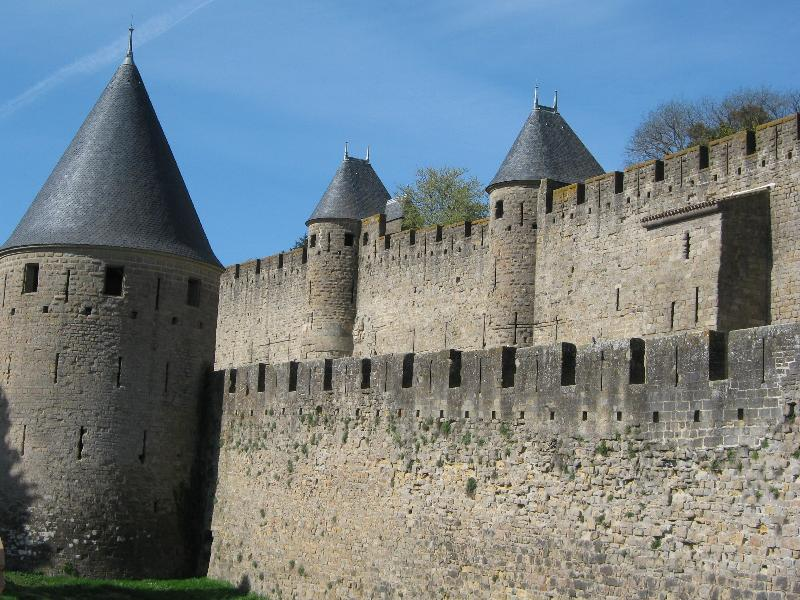
\includegraphics[width=0.95\textwidth]{assets/homography/castle_left}
    \end{minipage}%
    \hfill
    \begin{minipage}{.5\textwidth}
        \centering
    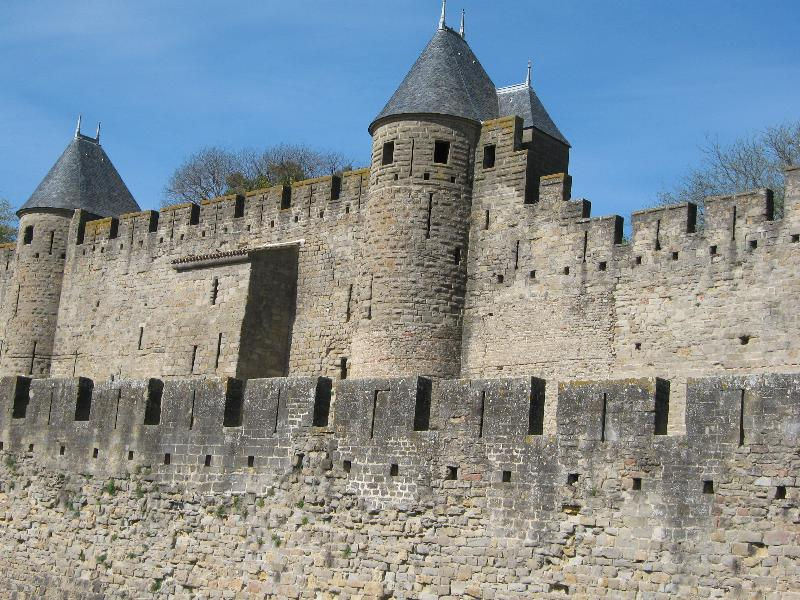
\includegraphics[width=0.95\textwidth]{assets/homography/castle_right}
    \end{minipage}
    \caption{The two input images.}
    \label{fig:castleimages}
\end{figure}

\begin{figure}[H]
    \centering
    \captionsetup{justification=centering}
    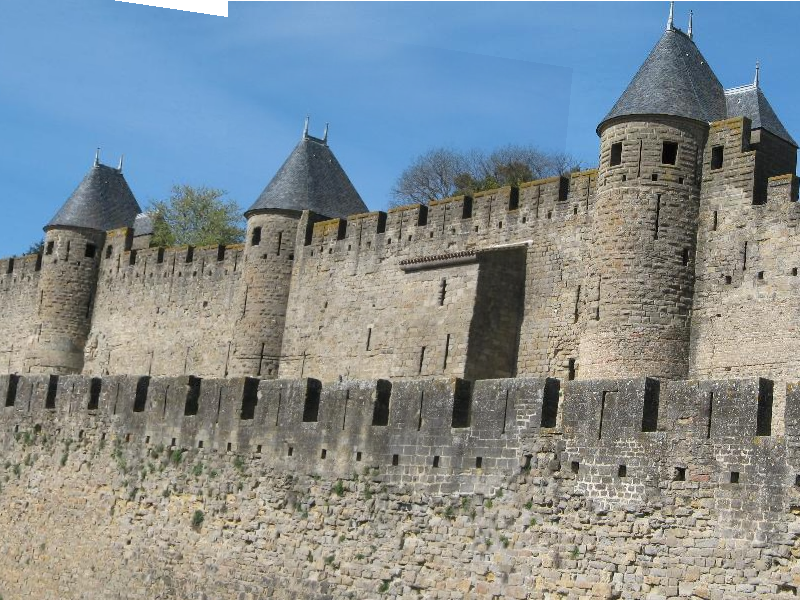
\includegraphics[width=0.475\textwidth]{assets/homography/castle_panorama}
    \caption{The stitched version of the images of figure~\ref{fig:castleimages} using paper~\citep{homography}.}
    \label{fig:panoramacastle}
\end{figure}

The homography matrix for the above stitching follows (\textit{QH.1}).

\[H=\left[
\begin{array}{c c c}
    1.16 & -0.11 & -525.59\\
    0.17 & 1.12 & -61.82\\
    2.18\times 10^{-4} & -2.89\times 10^{-5} & 1
\end{array}
\right]\]

As mentioned before, null values for $h_7$ and $h_8$ imply no change of perspective between the two images.
Here, $h_7$ and $h_8$ and are both very close to 0 which means that practically no perspective change occurred between
the two pictures of figure~\ref{fig:castleimages}, which seems plausible.

Comparatively, $h_3$ and $h_6$ are very large.
This is also plausible because they represent an overall translation in pixels (since $w'\approx 1$) and the images
are $800\times 600$.

The tool outputs not only the final panorama but also \textit{input images} and \textit{registered images}.

The input images 1 and 2 are simply the input images.
The registered images 1 and 2 are the two images that make up the final panorama.
That is, registered image 2 is simply the input image 2 but cropped (because the final panorama is of limited size
in this particular demo) and registered image 1 is the input image 1 but after the homography (and cropped as well).
This is because the authors decided to fix the second image and to warp the first one onto it: only the first image
is modified to build the panorama (\textit{QH.2}).

Taking the average of these two registered images pixel-wise gives the output panorama.

\begin{figure}[ht]
    \centering
    \captionsetup{justification=centering}
    \begin{minipage}{.5\textwidth}
        \centering
    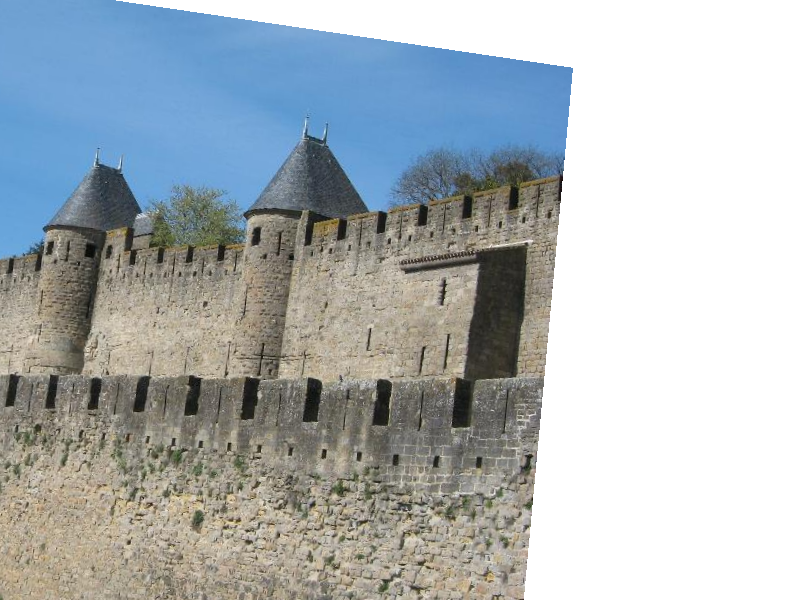
\includegraphics[width=0.95\textwidth]{assets/homography/reg_left}
    \end{minipage}%
    \hfill
    \begin{minipage}{.5\textwidth}
        \centering
    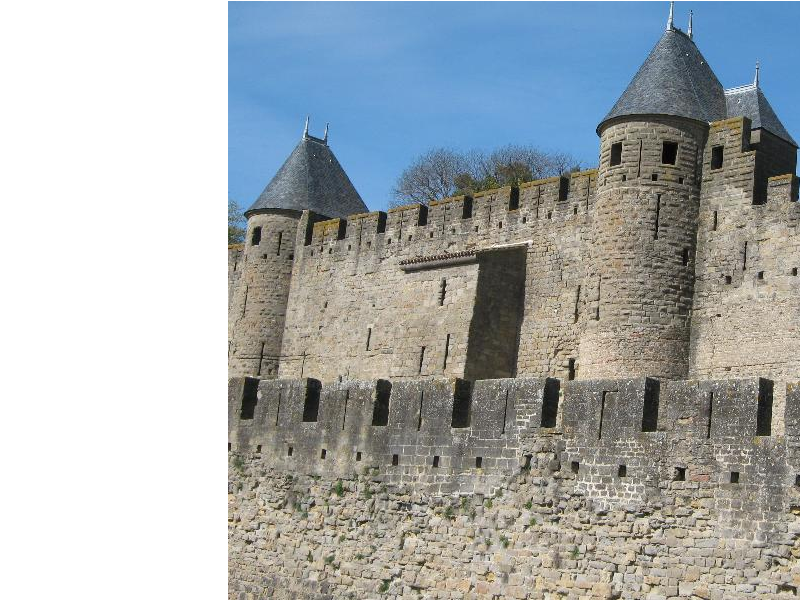
\includegraphics[width=0.95\textwidth]{assets/homography/reg_right}
    \end{minipage}
    \caption{The two \textit{registered} images.}
    \label{fig:regimages}
\end{figure}

The method used by the authors of~\citep{homography} is a modified RANSAC called ORSA (see figure~\ref{fig:orsa}).
They pick some set of points and compute the homography that best fits the points
(with the code of figure~\ref{fig:homographyfit}, \textit{QH.3}).

\begin{figure}[H]
    \centering
    \lstinputlisting[label={lst:orsa}]{assets/homography/orsa}
    \caption{(Simplified) code from~\citep{homography} that implements ORSA, their special RANSAC\@.}
    \label{fig:orsa}
\end{figure}

\begin{figure}[H]
    \centering
    \lstinputlisting[label={lst:homographyfit}]{assets/homography/homography_fit}
    \caption{(Simplified) code from~\citep{homography} to solve the system $Ah=0$.}
    \label{fig:homographyfit}
\end{figure}

For a specific set of $n$ points, they compute the homography and then the (ordered) vector of residues $(\epsilon_i)_i$
with $\epsilon_i = \left\|HP_i-P'_i\right\|_2$ where $P_i$ is the point in the left image and $P'_i$ the
corresponding point in the right image.
Using this vector of residues, they estimate the number of inliers using the $NFA$ (Number of False Alarms) which is a
measure of how likely it is to have these results if the number of inliers is $k$.
\[NFA=(n-4)\binom{n}{k}\binom{k}{4}\left(\epsilon_k^2\frac{\pi}{w'h'}\right)^{k-4}\]
The value of $k$ that minimizes this formula gives the number of inliers for the selected subset of points.

The $NFA$ (with optimized number of inliers $k$) also gives the measure of quality of $H$.
Hence, at each step, the homography with the smallest $NFA$ is kept (\textit{QH.4}).

Using this technique, we were able to stitch together four images into a larger panorama
(figure~\ref{fig:homography_img_1_2_3_4}, \textit{QH.5}).

\begin{figure}[ht]
    \centering
    \captionsetup{justification=centering}
    \begin{minipage}{.25\textwidth}
        \centering
    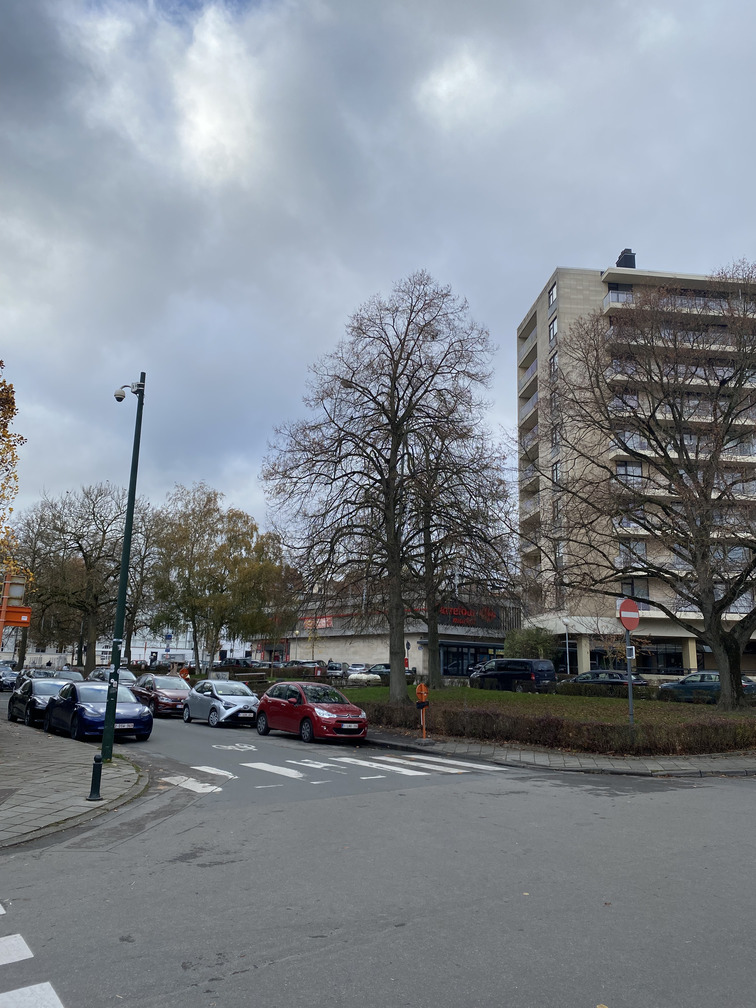
\includegraphics[width=0.95\textwidth]{assets/homography/img_1}
    \end{minipage}%
    \hfill
    \begin{minipage}{.25\textwidth}
        \centering
    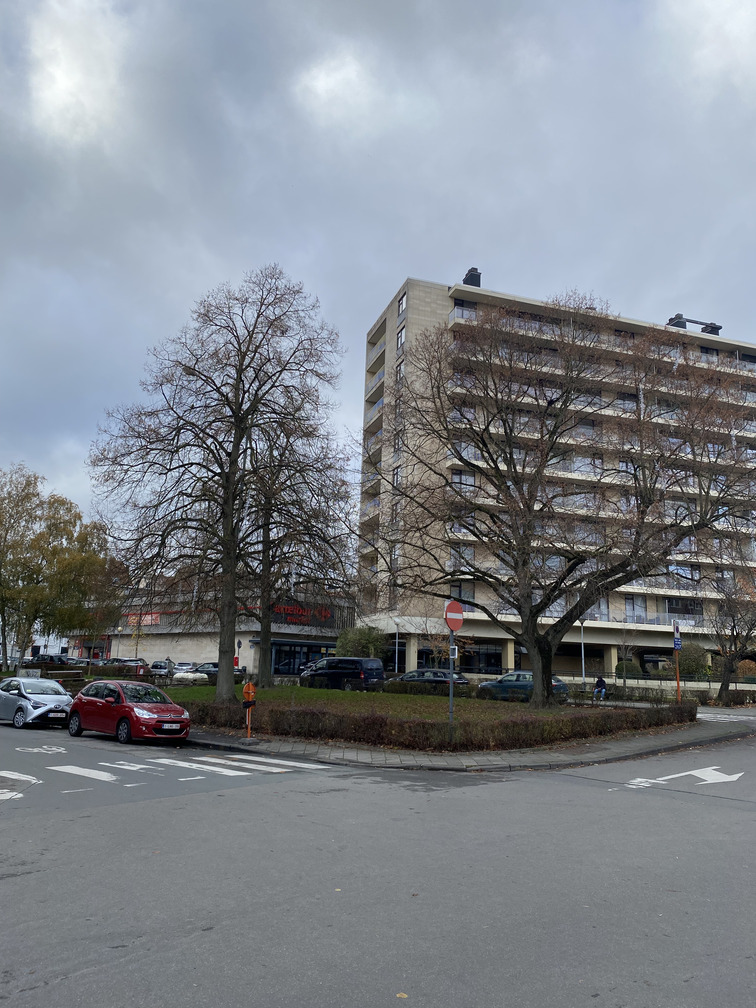
\includegraphics[width=0.95\textwidth]{assets/homography/img_2}
    \end{minipage}%
    \begin{minipage}{.25\textwidth}
        \centering
    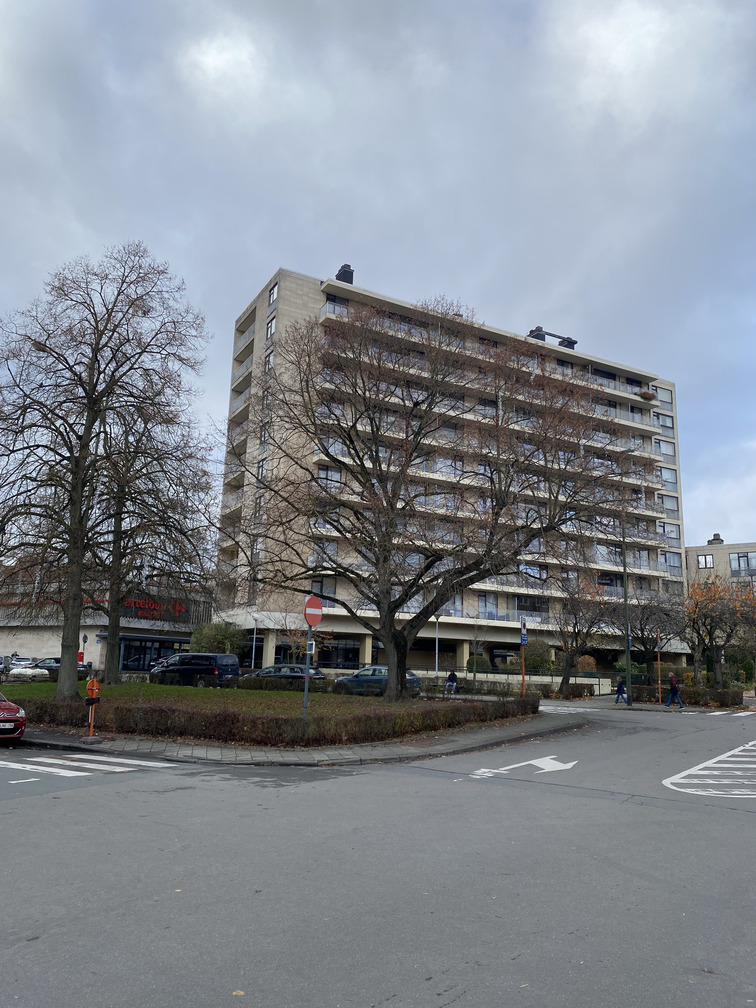
\includegraphics[width=0.95\textwidth]{assets/homography/img_3}
    \end{minipage}%
    \hfill
    \begin{minipage}{.25\textwidth}
        \centering
    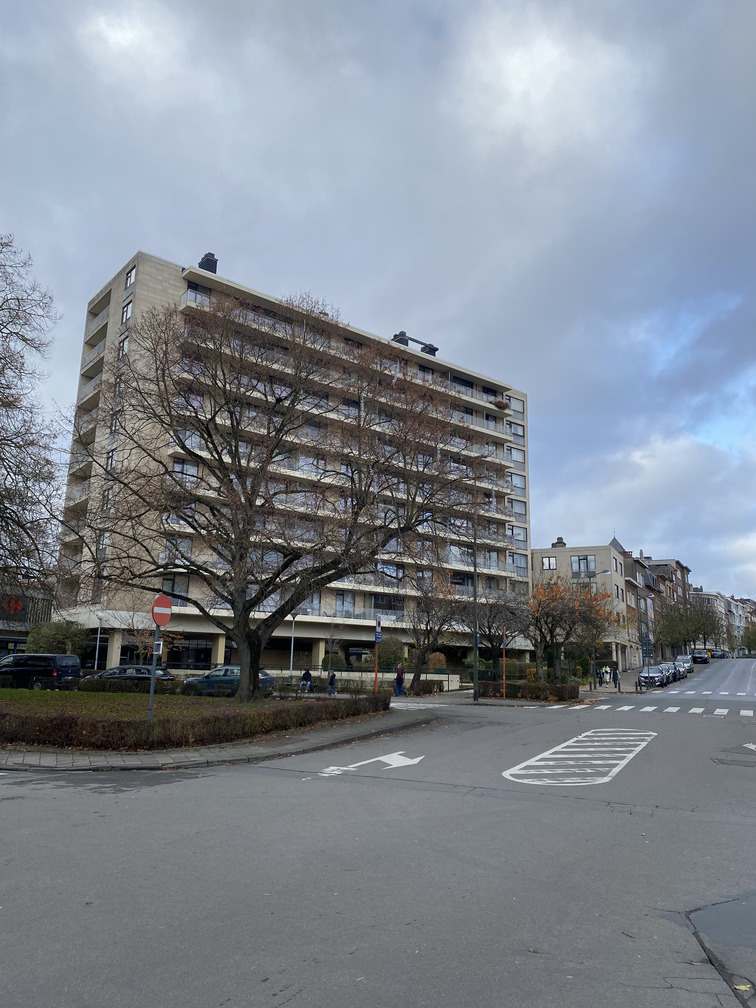
\includegraphics[width=0.95\textwidth]{assets/homography/img_4}
    \end{minipage}
    \caption{All images to be stitched.}
    \label{fig:homography_img_1_2_3_4}
\end{figure}

Using the online tool provided with the IPOL paper~\citep{homography}, we were able to find the homography matrices to
first stitch images 1 and 2, then images 3 and 4 and finally the two already stitched images into a full panorama.
We had to extract the homography matrices and perform the homography ourselves because the online tool crops the
resulting images to fit in the same frame as the input images.

\begin{figure}[ht]
    \centering
    \captionsetup{justification=centering}
    \begin{minipage}{.33\textwidth}
        \centering
    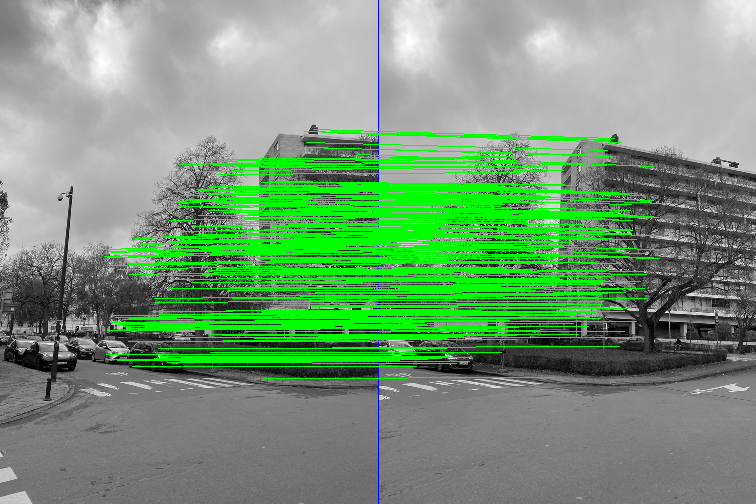
\includegraphics[width=0.95\textwidth]{assets/homography/img_12_inliers}
    \end{minipage}%
    \hfill
    \begin{minipage}{.33\textwidth}
        \centering
    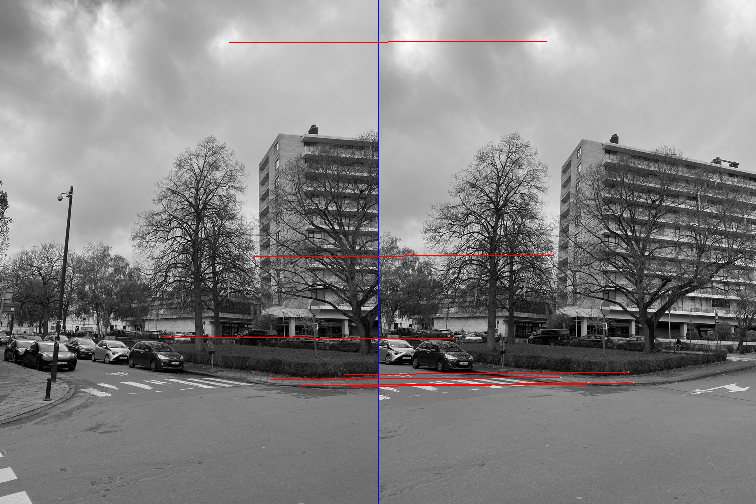
\includegraphics[width=0.95\textwidth]{assets/homography/img_12_outliers}
    \end{minipage}%
    \begin{minipage}{.33\textwidth}
        \centering
    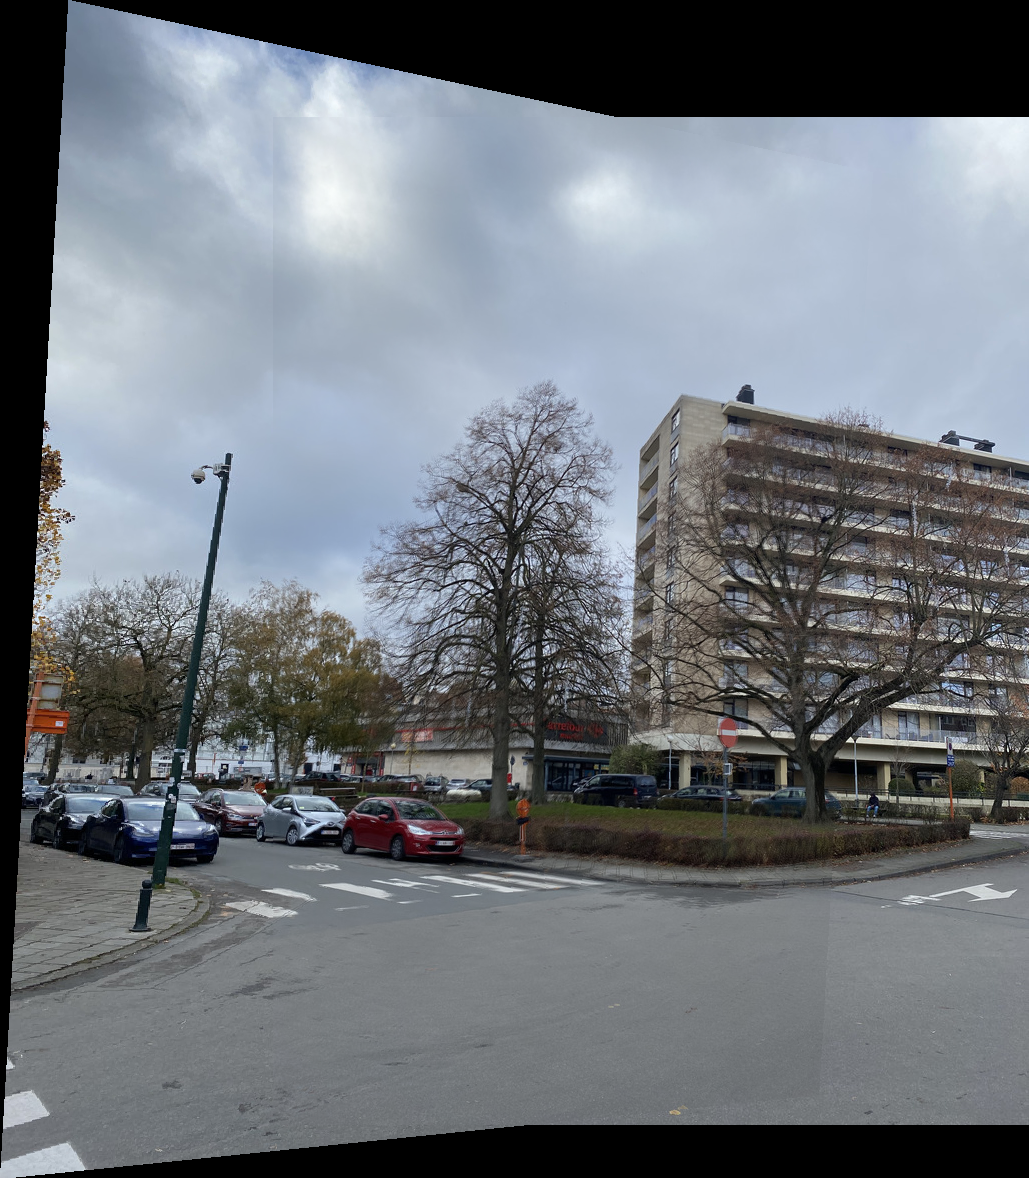
\includegraphics[width=0.95\textwidth]{assets/homography/img_12}
    \end{minipage}
    \caption{Stitched images 1 and 2 alongside the detected inliers and outliers.}
    \label{fig:homography_img_12}
\end{figure}

\begin{figure}[ht]
    \centering
    \captionsetup{justification=centering}
    \begin{minipage}{.33\textwidth}
        \centering
    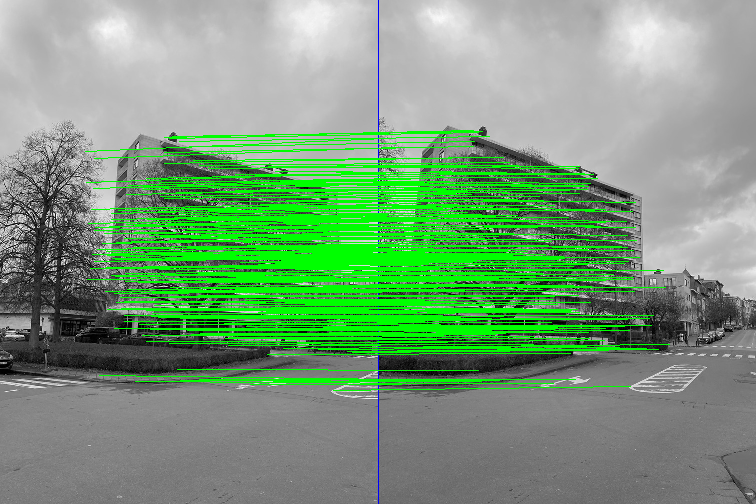
\includegraphics[width=0.95\textwidth]{assets/homography/img_34_inliers}
    \end{minipage}%
    \hfill
    \begin{minipage}{.33\textwidth}
        \centering
    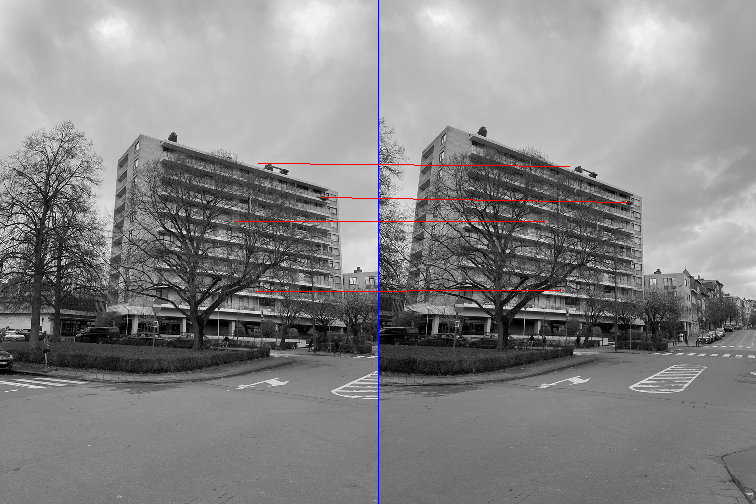
\includegraphics[width=0.95\textwidth]{assets/homography/img_34_outliers}
    \end{minipage}%
    \begin{minipage}{.33\textwidth}
        \centering
    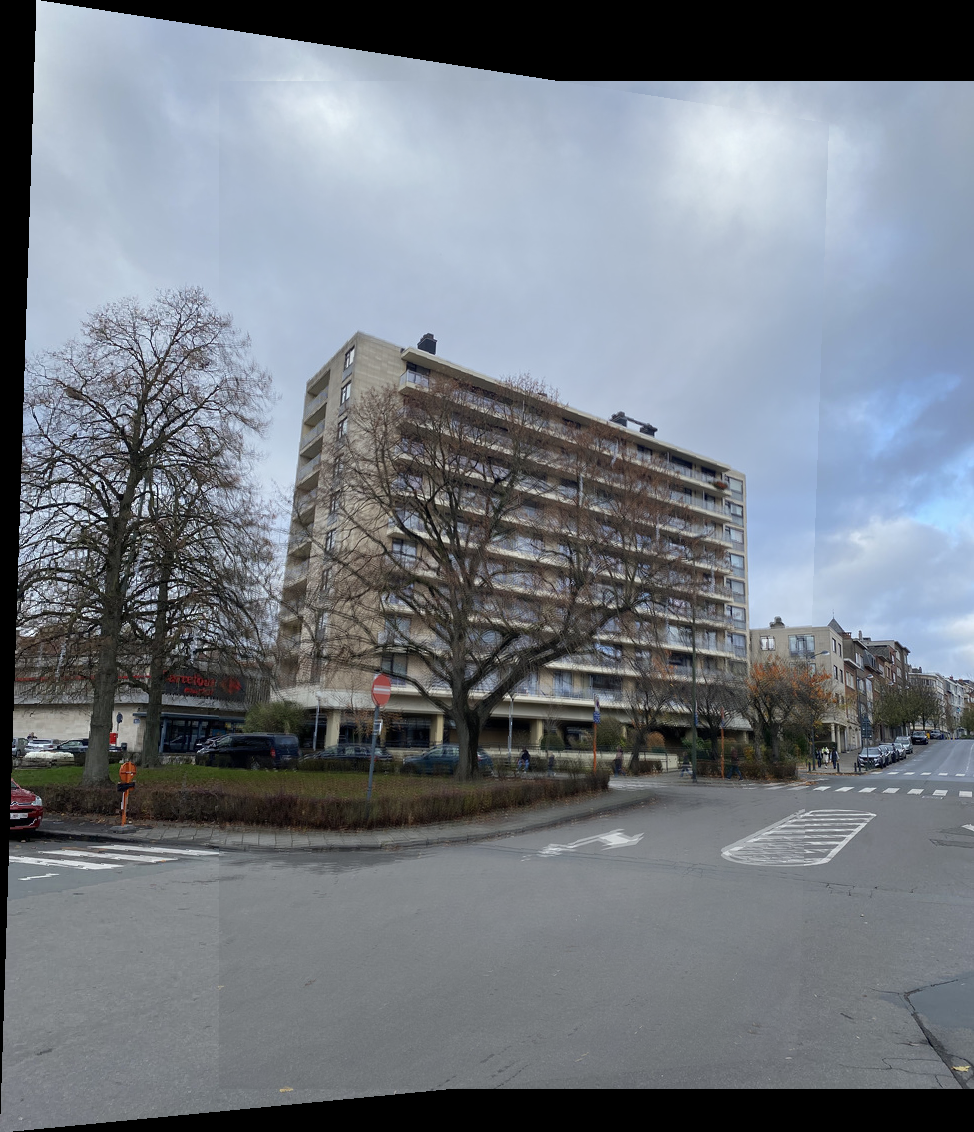
\includegraphics[width=0.95\textwidth]{assets/homography/img_34}
    \end{minipage}
    \caption{Stitched images 3 and 4 alongside the detected inliers and outliers.}
    \label{fig:homography_img_34}
\end{figure}

In both figures~\ref{fig:homography_img_12} and~\ref{fig:homography_img_34}, we can observe that the stitching is
blurry on points that are close to the camera (the roads).
This is because homography for stitching only works with flat scenes (or far away scenes).

\begin{figure}[ht]
    \centering
    \captionsetup{justification=centering}
    \begin{minipage}{.5\textwidth}
        \centering
    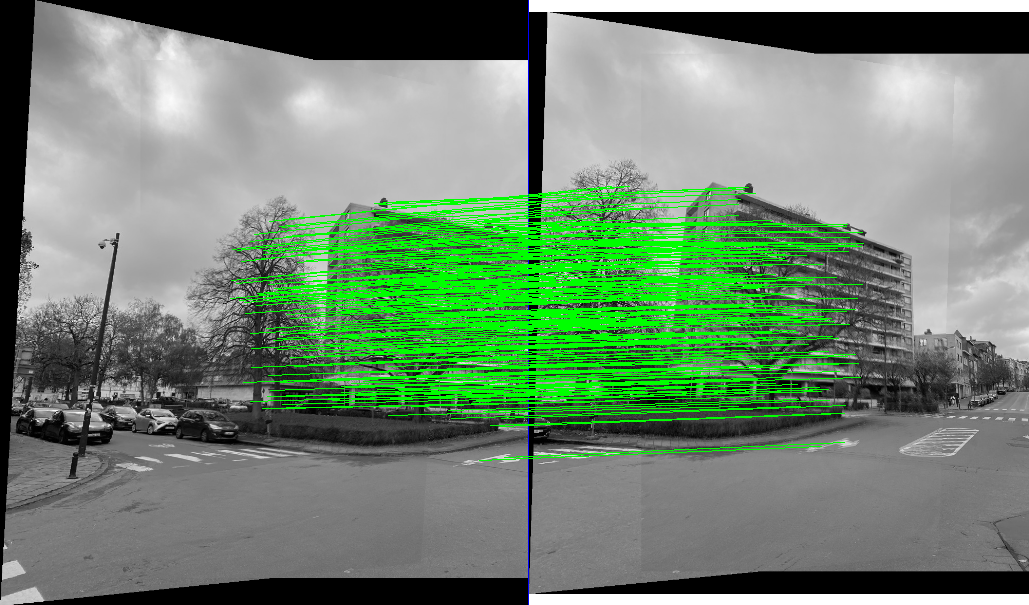
\includegraphics[width=0.95\textwidth]{assets/homography/img_1234_inliers}
    \end{minipage}%
    \hfill
    \begin{minipage}{.5\textwidth}
        \centering
    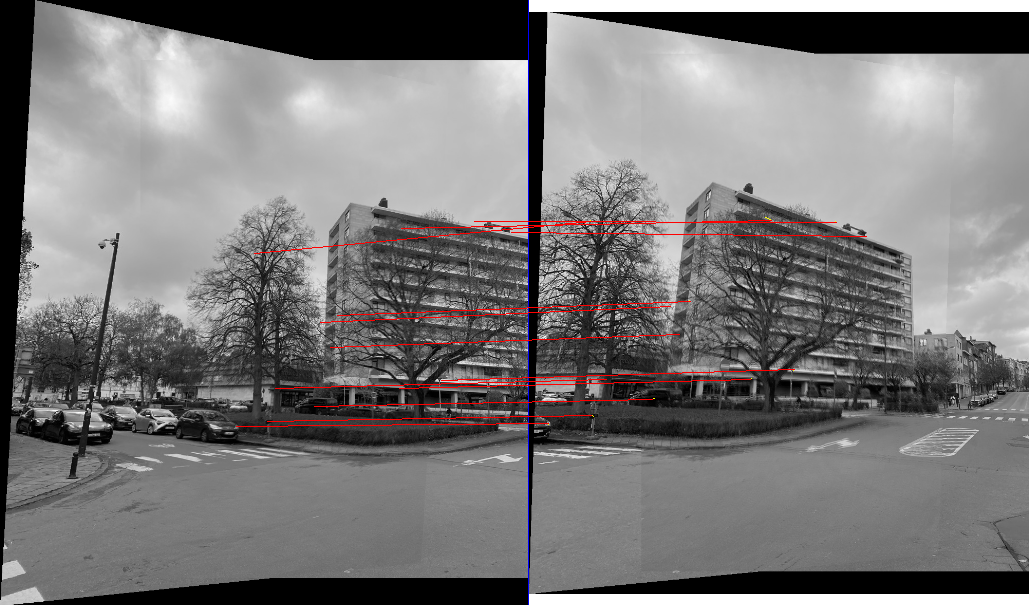
\includegraphics[width=0.95\textwidth]{assets/homography/img_1234_outliers}
    \end{minipage}
    \label{fig:homography_inliers_img_1234}
\end{figure}

\begin{figure}[ht]
    \centering
    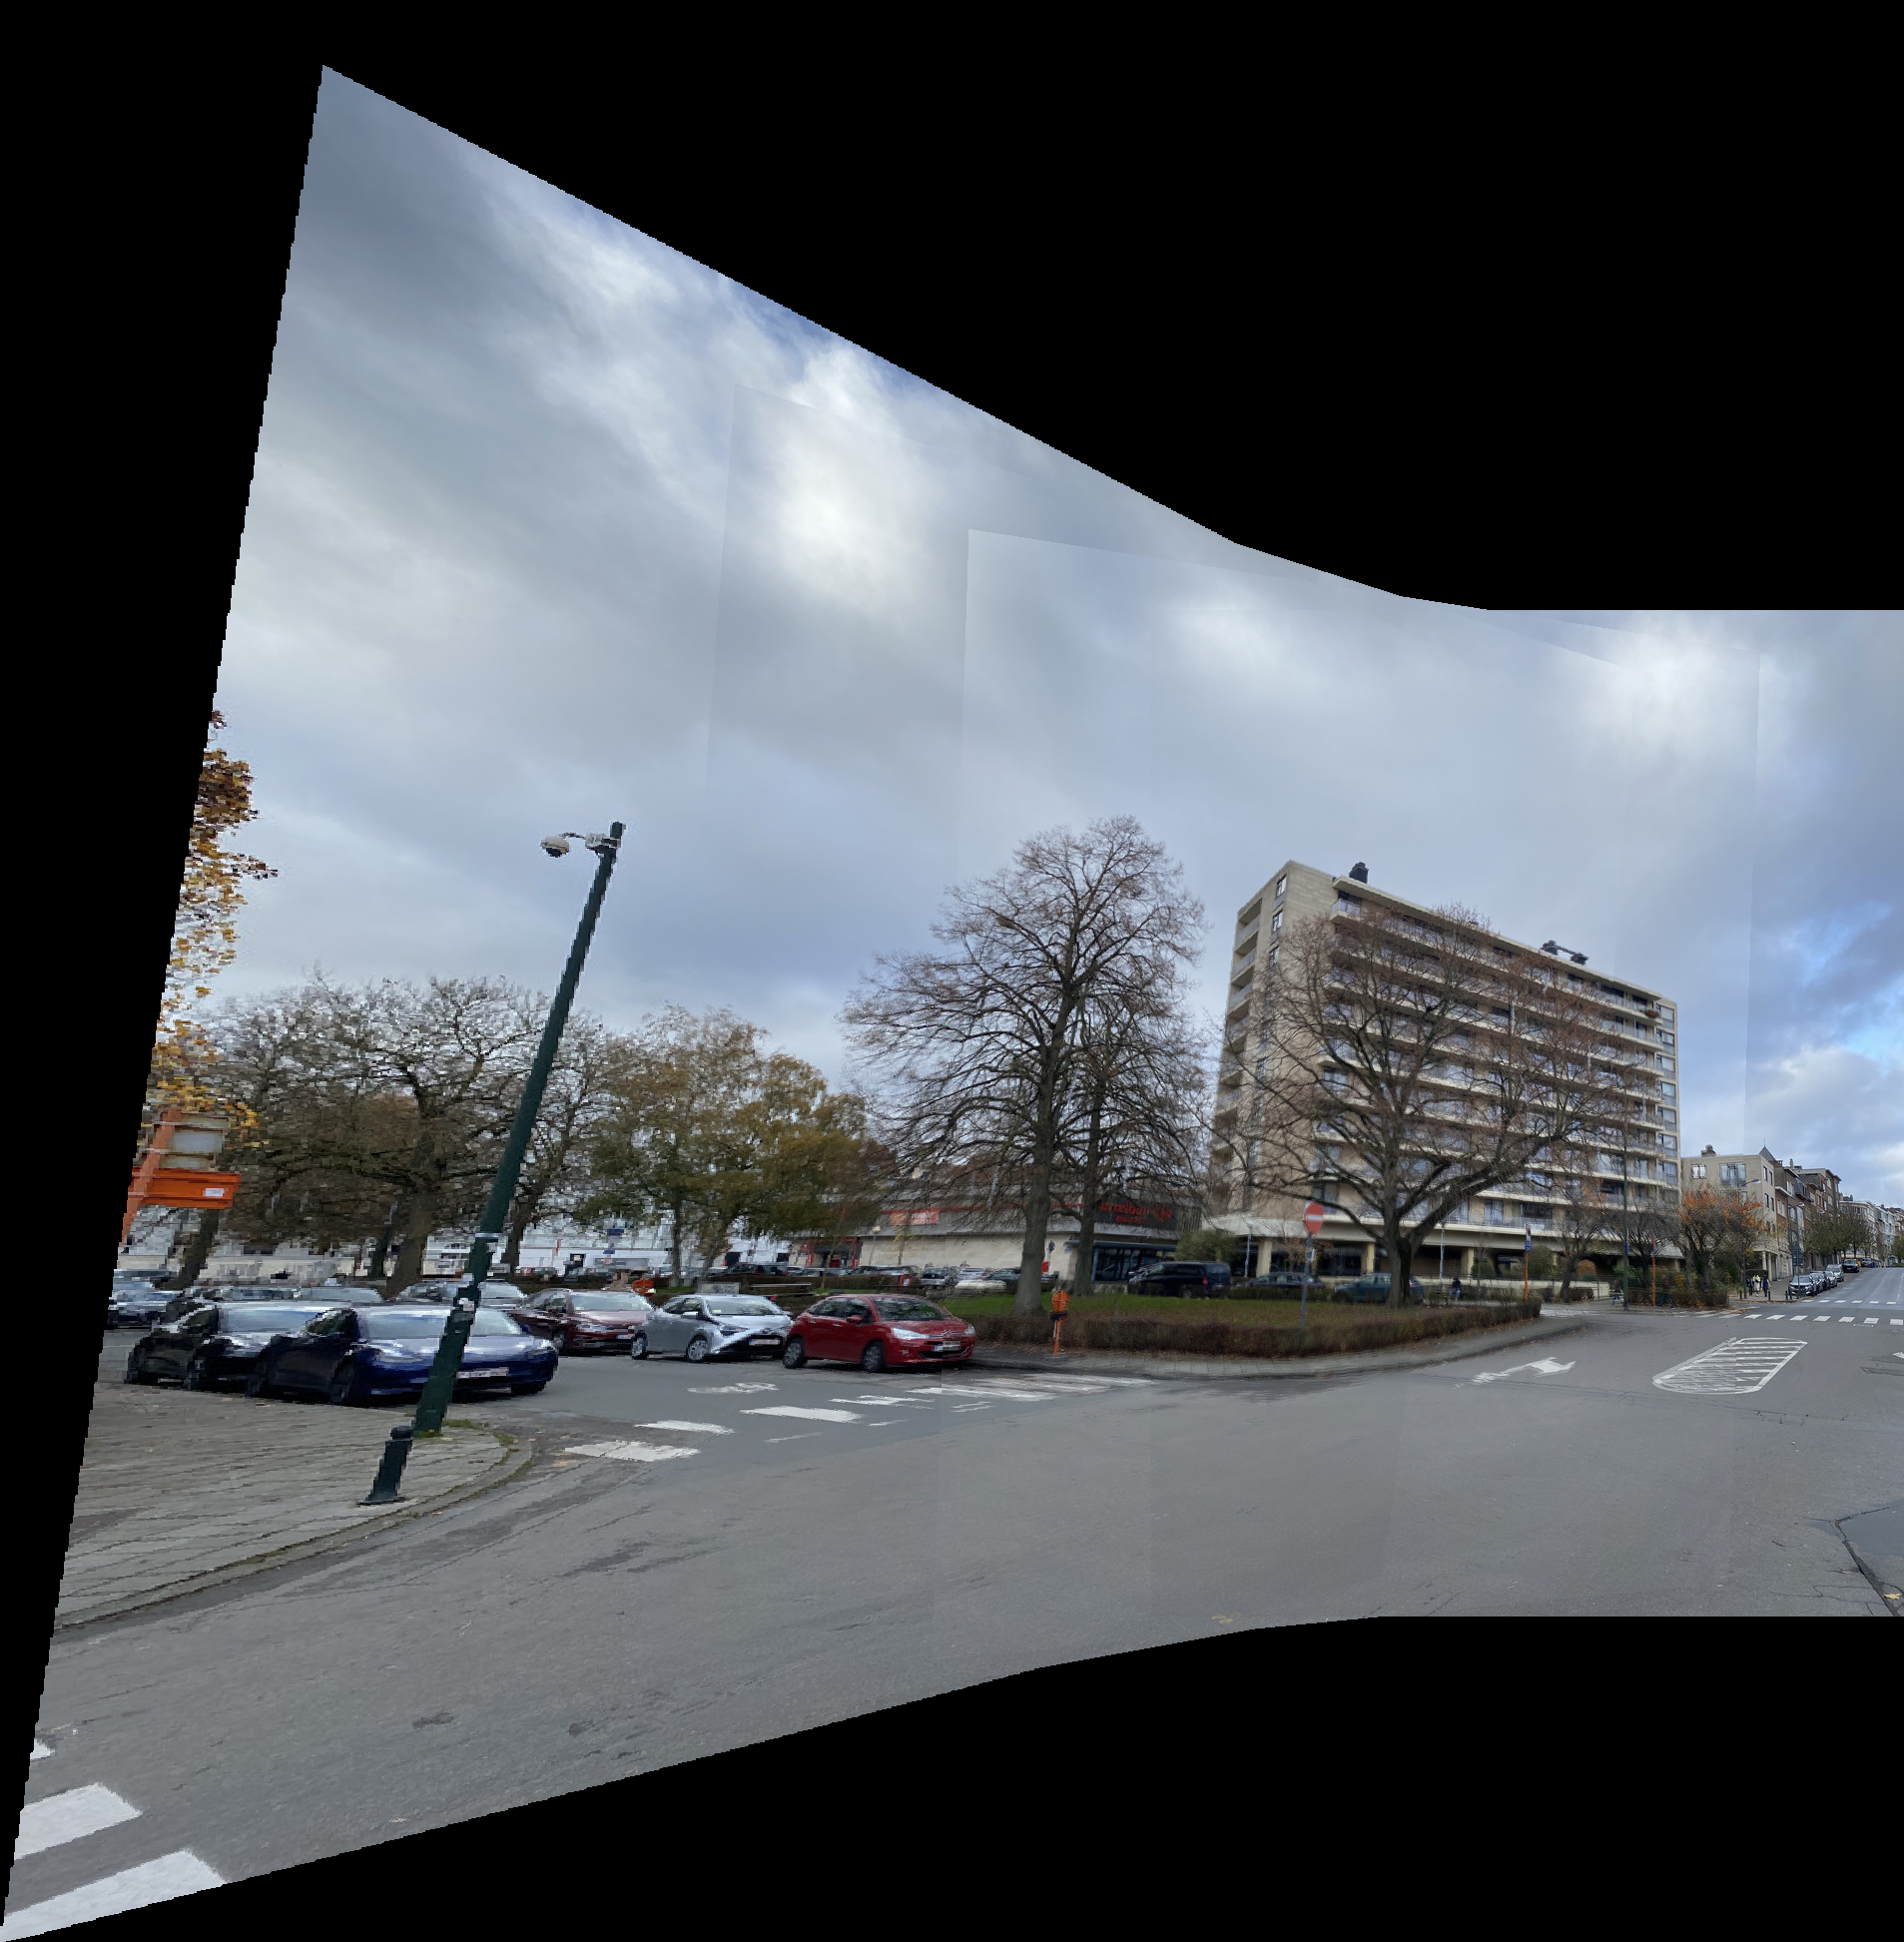
\includegraphics[width=0.65\textwidth]{assets/homography/img_1234}
    \caption{The final stitched panorama.}
    \label{fig:homography_img_1234}
\end{figure}

As we can observe in figure~\ref{fig:homography_img_1234}, the leftmost image was repeatedly distorted and became less
detailed.

For the sake of completeness, we provide the homography matrices found for each stitching.

\begin{gather*}
    \begin{array}{c c}
      H_{12}=\left[
\begin{array}{c c c}
    1.284 & -0.068 & -204.83\\
    0.248 & 1.17 & -116.55\\
    0.000367 & 0.000000189 & 1
\end{array}
\right] &
      H_{34}=\left[
\begin{array}{c c c}
    1.222 & -0.037 & -182.31\\
    0.175 & 1.127 & -81.10\\
    0.000285 & 0.00000303 & 1
\end{array}
\right]\end{array}\\
    H_{1234}=\left[
\begin{array}{c c c}
    2.037 & -0.123 & -782.54\\
    0.583 & 1.644 & -530.255\\
    0.000821 & -0.00000562 & 1
\end{array}
\right]
\end{gather*}